\section{Biographie du D\'eveloppeur}\label{chap:biographie}
\vspace{-0.9em}

\begin{center}
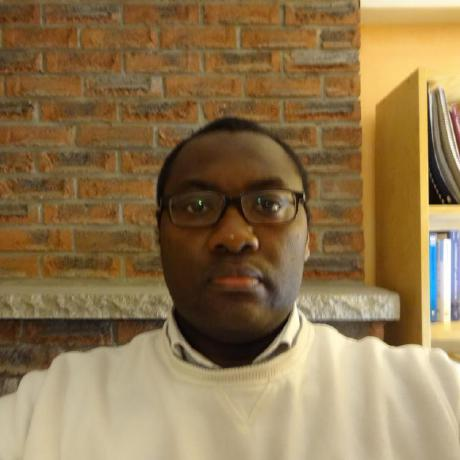
\includegraphics[scale=0.32]{../../francais/images/XavierNOUNDOU-2}
\captionof{figure}{Portrait du DR. XAVIER.\label{fig:xaviernoumbis}}
\end{center}

\textbf{\myfullacademicname} est CHR\'ETIEN de confession
(\'eglise \'evang\'elique du cameroun),
Camerounais, n\'e le $16$~Septembre $1983$ \`a
DOUALA (r\'egion du LITTORAL, CAMEROUN).

Le DR. Xavier est \textit{DOCTEUR/PH.D. en G\'enie Informatique}
(construction du logiciel, et test) depuis les $18$~Novembre~$2020$
gr\^ace a ses r\'esultats probants dans l'ing\'enierie
professionnelle du logiciel (\yerotherpblack), et de la recherche
fondamentale en g\'enie informatique (v\'erification statique
du code \cplusplus):

\begin{enumerate}
%	\itemsep -0.7em
	\item 'Context-Sensitive Staged Static Taint Analysis
			For C using LLVM'
		\begin{enumerate}[1.]
			\itemsep -0.7em
			\item code source en \cplusplus: \url{http://github.com/sazzad114/saint}
			\item texte complet (publi\'e le $1^\text{er}$~Juillet, $2015$): \url{http://archive.org/details/saint_201507}.
		\end{enumerate}		 

	\item 'YEROTH-ERP-3.0': \url{http://archive.org/details/yeroth-erp-3-0-info-english}.\\
\end{enumerate}


LE DR. XAVIER A $1$ GRADE ACAD\'EMIQUE ET PROFESSIONNELLE
DE ''DIPLOM--INFORMATIKER~(DIPL.--INF.)''
(ING\'ENIEUR DE CONCEPTION EN INFORMATIQUE) de
\textbf{l'\bremenu, BR\^EME, BREMEN, ALLEMAGNE}
($25$~MAI~$2007$).

